\chapter{The Robot Models}
\label{cha:robots}

%Later: HOAP-2, NEC Papero (I already did a model in Blender), CITIZEN Eco-Be!, VisiON 4g (Fabio Dalla Libera is working on that), AIBO via RoSIML importer

Below, we only describe the most advanced robot model that comes with the simulation package at this point in time: the Soccerbot. There are some other models which you can find in the directory \texttt{rcssserver3d/data/rsg/agent/}, e.g., the soccerplayer.rsg, or the hoap2.rsg files. These are currently not in use in any simulation, and considered experimental.

Besides that, work is in progress on other robot models and will be described here when usable. We plan to integrate an improved model of the HOAP-2 robot from Fujitsu Automation, and models of the VisiON 4g robot, and the Sony AIBO. For help on how to model new robots for your simulation, please have a look at tutorials in the SimSpark Wiki at \\

\url{http://simspark.sourceforge.net/wiki/}.

\section{Soccerbot}

This is the robot currently used in the competitions of the 3D Soccer Simulation League at RoboCup. It is a humanoid robot with 20 degrees of freedom (DOF) as depicted in figure \ref{fig:soccerbotdof}. Its current dimensions are quite unrealistic for a real humanoid robot (see table \ref{table:dimensions} which is due to instabilities in the physics simulation at the time the robot was first modeled. This is a serious shortcoming of this robot model and should be changed. Another open issue is that the joint ranges are not limited in the current model. This allows for very unrealistic movements which can be fun to watch, but can lead to unfair behavior in a competition.

\begin{figure}[htp]
\begin{minipage}[b]{0.5\linewidth} 
\centering
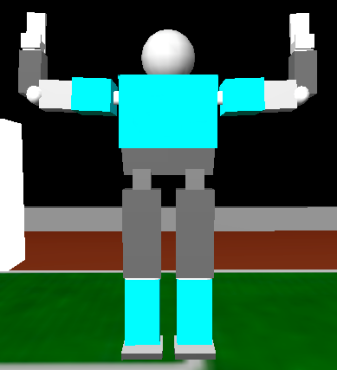
\includegraphics[width=6cm]{fig/soccerbotfront}
\caption{Frontal view of the Soccerbot in the simulation}
\end{minipage}
\hspace{0.5cm}
\begin{minipage}[b]{0.5\linewidth}
\centering
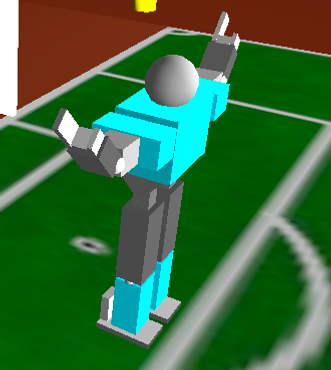
\includegraphics[width=6cm]{fig/soccerbotside}
\caption{Side view of the Soccerbot in the simulation}
\end{minipage}
\end{figure}

\begin{figure}[htp]
  \centering
  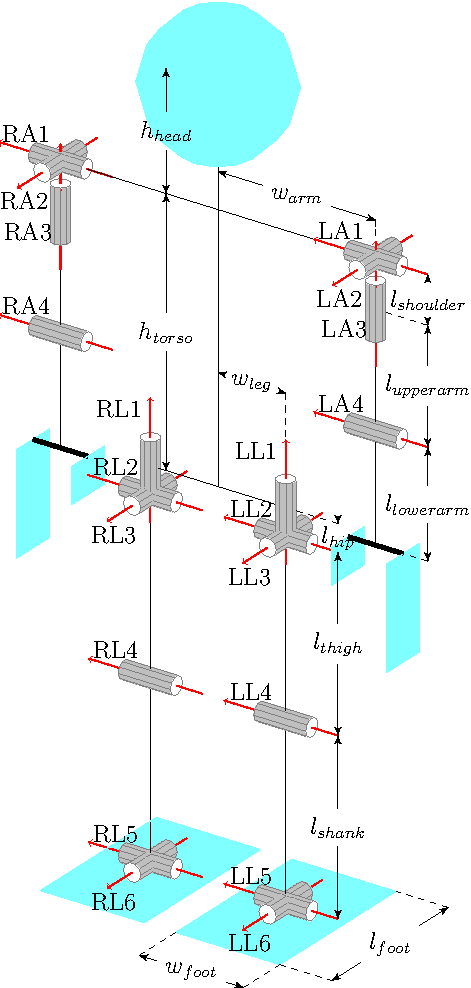
\includegraphics[height=0.6\textwidth]{fig/soccerbot056}
  \caption{Overview of the degrees of freedom of the Soccerbot}
  \label{fig:soccerbotdof}
\end{figure}

\begin{table}
\centering
\begin{tabular}[htbp]{|l|c|c|c|c|}
  \hline
  Name & Width & Depth & Height & Mass \\
  \hline\hline
  head & \multicolumn{3}{|c|}{0.39m (radius)} & 0.3kg\\ \hline
  torso & 1.37m & 0.96m & 1.41m & 1.8kg \\ \hline
  left\_shoulder & 0.445m & 1.017m & 0.536m & 0.5kg \\ \hline
  right\_shoulder & 0.445m & 1.017m & 0.536m & 0.5kg \\ \hline
  left\_upper\_arm & 0.445m & 0.398m & 0.506m & 0.2kg \\ \hline
  right\_upper\_arm & 0.445m & 0.398m & 0.506m & 0.2kg \\ \hline
  left\_lower\_arm & 0.445m & 0.316m & 0.6m & 0.2kg \\ \hline
  left\_lower\_arm & 0.445m & 0.316m & 0.6m & 0.2kg \\ \hline
  left\_hip & 0.273m & 0.273m & 0.2m & 0.1kg \\ \hline
  right\_hip & 0.273m & 0.273m & 0.2m & 0.1kg \\ \hline
  left\_thigh & 0.56m & 0.56m & 1.3m & 0.25kg \\ \hline
  right\_thigh & 0.56m & 0.56m & 1.3m & 0.25kg \\ \hline
  left\_shank & 0.56m & 0.56m & 0.964m & 0.25kg \\ \hline
  right\_shank & 0.56m & 0.56m & 0.964m & 0.25kg \\ \hline
  left\_foot & 0.6m & 0.956m & 0.095m & 0.1kg \\ \hline
  right\_foot & 0.6m & 0.956m & 0.095m & 0.1kg \\
  \hline
\end{tabular}
\caption{Physical properties of the Soccerbot.}
\label{table:dimensions}
\end{table}%

The Soccerbot has several kinds of sensors available. It uses a (omni-directional) vision sensor (see section \ref{sec:visionperceptor}) to get information about objects in its environment\footnote{It is currently located in the center of the torso, which should be changed to be in the head.}. In order to detect the contact with the ground and the resulting force at the feet, it is equipped with a Force Resistance Perceptor (see section \ref{sec:FRP}) in each foot. It can sense the current simulation time with a GameState Perceptor (see section \ref{sec:gamestateperceptor}) and the change in orientation of its torso with a GyroRate Perceptor (see section \ref{sec:GYR}). Furthermore, it has proprioceptive sensors that allow to sense the angle of each joint (see sections \ref{sec:HJP} and \ref{sec:UJP} for HingeJoint Perceptor and UniversalJoint Perceptor descriptions, respectively). An overview over the joint perceptors and effectors is given in table \ref{table:perceptorNames}.

\begin{table}
\label{table:perceptorNames}
\caption{Perceptor and effector names}
\begin{center}
\begin{tabular}{|l|l|l|l|}
\hline
{\bf Connection between}  & {\bf Joint type} & {\bf Perceptor name}& {\bf
Effector name} \\
\hline
Shoulder - body  & Universal joint & laj1\_2  raj1\_2 & lae1\_2   rae1\_2 \\
\hline
Upper arm - shoulder  & Hinge joint & laj3  raj3 & lae3   rae3 \\
\hline
Forearm - upper arm  & Hinge joint & laj4  raj4 & lae4   rae4 \\
\hline
Hip - body  & Hinge joint & llj1  rlj1 & lle1   rle1 \\
\hline
Upper leg - hip & Universal joint & llj2\_3  rlj2\_3 & lle2\_3   rle2\_3 \\
\hline
Lower leg - upper leg & Hinge joint & llj4  rlj4 & lle4   rle4 \\
\hline
foot - lower leg & Universal joint & llj5\_6  rlj5\_6 & lle5\_6   rle5\_6 \\
\hline
\end{tabular}
\end{center}
\end{table}

In figure \ref{fig:examplemsg} shows an example message which the agent receives from the server in a single simulation cycle including sense information from all the perceptors of the agent.

\begin{figure}[htb]
\centering
\parbox{\textwidth}{
\texttt{
(time (now 19.60))(GYR (n torso) (rt -0.02 -0.01 -0.00))(See (F1L (pol 10.34 45.02 -16.70)) (F2L (pol 68.43 174.14 -2.56)) (F1R (pol 103.28 -86.10 -1.66)) (F2R (pol 123.46 -123.42 -1.43)) (G1L (pol 27.94 165.40 -6.96)) (G2L (pol 35.03 168.43 -5.56)) (G1R (pol 106.49 -104.59 -1.83)) (G2R (pol 108.57 -108.33 -1.80)) (B (pol 56.95 -122.42 -3.02)) (P (team RoboLog) (id 2) (pol 10.50 -179.98 -0.07)))(UJ (n laj1\_2) (ax1 0.00) (ax2 90.63))(UJ (n raj1\_2) (ax1 -0.00) (ax2 90.63))(HJ (n laj3) (ax 90.77))(HJ (n raj3) (ax -90.77))(HJ (n laj4) (ax 87.96))(HJ (n raj4) (ax 88.40))(HJ (n llj1) (ax 0.03))(HJ (n rlj1) (ax -0.02))(UJ (n llj2\_3) (ax1 -0.03) (ax2 0.02))(UJ (n rlj2\_3) (ax1 -0.02) (ax2 0.01))(HJ (n llj4) (ax 0.05))(HJ (n rlj4) (ax 0.04))(TCH (n lf) (val 1))(UJ (n llj5\_6) (ax1 0.05) (ax2 -0.01))(TCH (n rf) (val 1))(UJ (n rlj5\_6) (ax1 0.04) (ax2 -0.00))}
}
\caption{An example message from the server to the Soccerbot including information from all the sensors.}
\label{fig:examplemsg}
\end{figure}

\section{Nao}
\label{sec;nao}
The Nao humanoid robot manufactured by Aldebaran Robotics. Its height
is about 57cm and its weight is around 4.5Kg. Its biped architecture
with 22 degrees of freedom allows Nao to have great mobility. The
rcssserver3D can simulate the Nao robot nicely, see \autoref{fig:nao}.
\begin{figure}[htp]
  \centering
  \def\mheight{5cm}
  \subfigure[real robot]{
    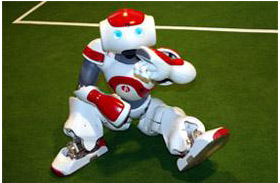
\includegraphics[height=\mheight]{fig/realNao}
  }
  \subfigure[virtual robot]{
    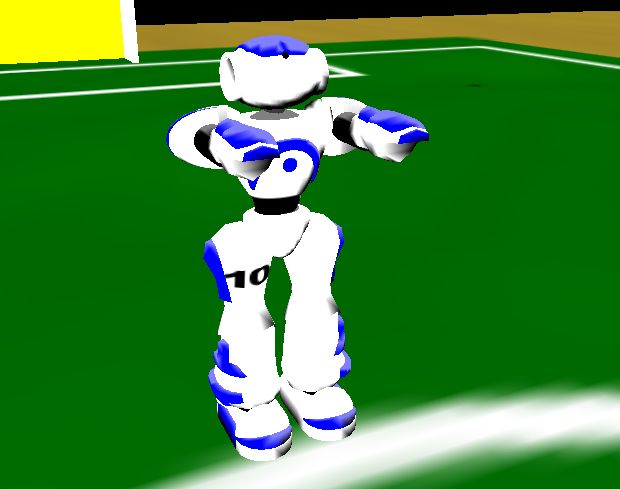
\includegraphics[height=\mheight]{fig/virtualNao}
  }
  \caption{The Nao humanoid robot}
  \label{fig:nao}
\end{figure}

\subsection{Parameters}
This section is quite important to the agent development for the
parameters used to construct the robot are showed in this section.
Firstly, \autoref{fig:naojoints} is a picture shows how the joints
move. Second, \autoref{tab:nao-conf} shows the detailed parameters.
\begin{figure}[htp]
  \centering
  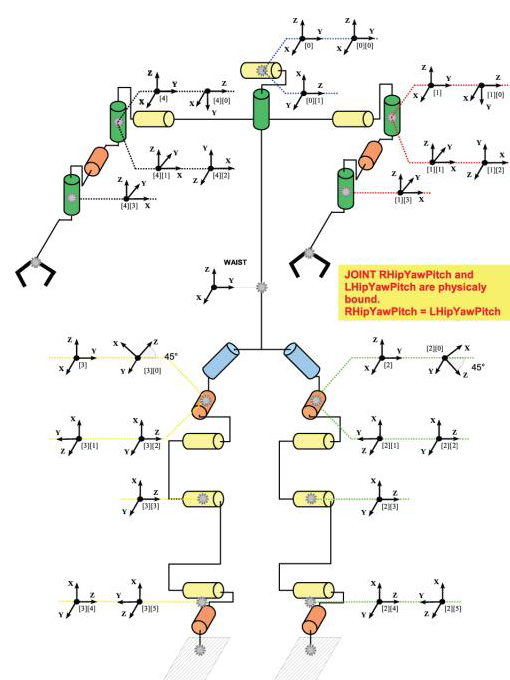
\includegraphics[width=0.618\textwidth]{fig/naojoints}
  \caption{The joints of Nao robot}
  \label{fig:naojoints}
\end{figure}

\begin{landscape}
\begin{table}
  \centering
  \label{tab:nao-conf}
  \caption{Configuration of Nao (see the text for the meaning of each
    column)}
  \newcommand{\threegrid}[1]{\multicolumn{3}{c|}{#1}}
  \newcommand{\fourgrid}[1]{\multicolumn{4}{c|}{#1}}
  \begin{tabular}{|l|l|r@{,}r@{,}r@{}c|l|l|l|r@{,}r@{,}r|r@{,}r@{,}l@{}c|l|l|}
    \hline
    {\bf Name} & {\bf Parent} & \fourgrid{\bf Translation} &
    {\bf Mass} & {\bf Geometry} & {\bf Name} & \threegrid{\bf
      Anchor} & \fourgrid{\bf Axis} & {\bf Min} & {\bf Max} \\
    \hline
    neck & torso & 0&0&0.09& & 0.05 & Cylinder & HJ1 & 0&0&0 & 0&0&1& &
    -120 & 120\\
    & & \fourgrid{} & & L: 0.08 R: 0.015 & & \threegrid{} & \fourgrid{} & &\\
    \hline
    head & neck & 0&0&0.065& & 0.35 & Sphere 0.065 & HJ2 & 0&0&-0.005 &
    1&0&0& & -45 & 45\\
    \hline
    shoulder & torso & 0.098&0&0.075&(r)  & 0.07 & Sphere 0.01& AJ1 &
    0&0&0 & 1&0&0& & -120 & 120 \\
    & & -0.098 & 0 & 0.075&(l) & & & & \threegrid{} & \fourgrid{} & & \\
    \hline
    upperarm & shoulder & 0.01&0.02&0&(r) & 0.150 &
    Box & AJ2 & \threegrid{-Translation} & 0&0&1& & -95(r) & 1(r)  \\
    & & -0.01 & 0.02 & 0&(l) & & 0.07, 0.08, 0.06 & & \threegrid{} & \fourgrid{} & -1(l) & 95(l) \\
    \hline
    elbow & upperarm & -0.01&0.07&0.009&(r) &
    0.035 & Sphere 0.01 & AJ3 & 0&0&0 & 0&1&0& & -120 & 120 \\
    & & 0.01 & 0.07 & 0.009&(l) & & & & \threegrid{} & \fourgrid{} & &\\
    \hline
    lowerarm & elbow & 0&0.05&0& & 0.2 & Box & AJ4 &
    \threegrid{-Translation} & 0&0&1& & -1(r) & 90(r) \\
    & & \fourgrid{} & & 0.05, 0.11, 0.05 & & \threegrid{} & \fourgrid{} & -90(l) & 1(l) \\
    \hline
    hip1 & torso & 0.055&-0.01&-0.115&(r) &
    0.09 & Sphere 0.01 & LJ1 & 0&0&0 & -0.7071&0&0.7071&(r)  & -90 & 1 \\
    & & -0.055 & -0.01 & -0.115&(l) & & & & \threegrid{} & -0.7071&0&-0.7071&(l) & &\\
    \hline
    hip2 & hip1 & 0&0&0& & 0.125 & Sphere 0.01 & LJ2 & 0&0&0 & 0&1&0& &
    -45(r) & 25(r)\\
    & & \fourgrid{} & & & & \threegrid{} & \fourgrid{} & -25(l) & 45(l) \\
    \hline
    thigh & hip2 & 0&0.01&-0.04& & 0.275 & Box & LJ3 &
    \threegrid{-Translation} & 1&0&0& &  -25 & 100\\
    & & \fourgrid{} & & 0.07, 0.07, 0.14 & & \threegrid{} & \fourgrid{} & & \\
    \hline
    shank & thigh & 0&0.005&-0.125& & 0.225 & Box  & LJ4
    & 0&-0.01&0.045 & 1&0&0& & -130 & 1\\
    & & \fourgrid{} & & 0.08, 0.07, 0.11 & & \threegrid{} & \fourgrid{} & &\\
    \hline
    ankle & shank & 0&-0.01&-0.055& & 0.125 & Sphere 0.01 & LJ5 & 0&0&0
    & 1&0&0& & -45 & 75\\
    \hline
    foot & ankle & 0&0.03&-0.035& & 0.2 & Box & LJ6 & 0&-0.03&0.035 & 0&1&0& & -25(r) & 45(r)\\
    & & \fourgrid{} & & 0.08, 0.16, 0.03 & & \threegrid{} & \fourgrid{} & -45(l) & 25(l)\\
    \hline
    Torso &  & \fourgrid{} & 1.2171 & Box & & \threegrid{} & \fourgrid{} & &\\
    & & \fourgrid{} & & 0.1, 0.1, 0.18 & & \threegrid{} & \fourgrid{} & &\\
    \hline
  \end{tabular}
\end{table}
\end{landscape}
Meaning of each column from left to right in \autoref{tab:nao-conf}
are explained as follow:
\begin{description}
\item[Name] the body part name of Nao
\item[Parent]  the parent of the body
\item[Translation] the offset relative to its parent
\item[Mass] the mass of this body
\item[Geometry] the size of its geometry representation
\item[Name] the joint name installed on this body
\item[Anchor] the offset of the joint anchor relative to the body that
  installed on
\item[Axis] the joint axis relative to the body that installed on
\item[Min] the min angle that the joint can reach
\item[Max] the max angle that the joint can reach
\end{description}

\subsection{Implementation}
The Nao robot model is implemented in the rsg files under
\texttt{rcssserver3d/data/rsg/agent/nao}, see \autoref{tab:nao-implement}
for details. This section goes much deeper and is a little boring.
\begin{table}[htp]
  \centering
  \caption{The rsg files of Nao robot}
  \label{tab:nao-implement}
  \begin{tabular}{lp{0.6\textwidth}}
    \hline
    {\bf File Name}             & {\bf Description} \\
    \hline
    box\_appearance.rsg         & Install a box which is for the GL
    render. \\
    box\_physics.rsg            & Install a box that has physics
    effect(ODE related) \\
    box\_physics\_nocollider.rsg & Install a box that only has dynamics
    effect (mass, linear velocity, etc). But it can never collide to
    the others. \\
    box\_physics\_with\_handler.rsg & Not only do the job as file
    “box\_physics.rsg”, but also install a touchperceptorhandler under
    the BoxCollider Node. \\
    ccylinder\_appearance.rsg   & Install a capped cylinder which is
    for the GL render. \\
    ccylinder\_physics.rsg      & Install a capped cylinder that has
    physics effect(ODE related) \\
    ccylinder\_physics\_nocollider.rsg & Install a capped cylinder that
    only has dynamics effect (mass, linear velocity, etc). But it can
    never collide to the others. \\
    contactjointhandler.rsg    & Install a contactjointhandler to
    handle the collisions. \\
    dragcontroller.rsg         & Install a DragController. \\
    goal.rsg                   & Install the goal. \\
    hingejoint.rsg             & Install a hingejoint. \\
    \hline
  \end{tabular}
\end{table}

%%% Local Variables: 
%%% mode: latex
%%% TeX-master: "user-manual"
%%% End: 
